\chapter{Sistema de grabación online}

Para poder obtener audios de distintas personas se desarrolló una página web. Esto nos da muchas ventajas ya que nos permite grabar fácilmente desde cualquier lugar. En esta sección explicaremos la arquitectura del sistema y sus detalles técnicos.

La página web está desarrollada en Django, versión 1.4.2. Se eligió este framework por su facilidad a la hora de guardar objetos a la base de datos y también por la cantidad importante de bibliotecas que posee Python. La versión de Python que se utilizó es 2.7.3. 

En la base de datos se guardó la información de cada hablante, las frases a grabar y las trazas. La base de datos elegida fue PostgreSQL versión 9.1 y se eligió esta ya que es de código abierto. Los archivos de audio se guardaron en archivos \textit{wav} por separado y se guardó una referencia al nombre del archivo generado en la base de datos. Para el servidor HTTP se utilizó Apache versión 2.2.22. El servidor utilizó el sistema operativo Ubuntu 12.04.4 LTS.

\section{Recolección de datos}

Cuando un usuario visitó nuestra página, primero debió llenar un formulario. Este le pregunta: género, fecha de nacimiento, lugar donde se crió y donde reside actualmente. Al confirmar el formulario, estos son grabados en la base de datos de la aplicación en el servidor. Esto se puede apreciar en la Figura \ref{figEncuesta}. Luego se procede a realizar las grabaciones. 

\begin{figure}[h!]
    \centerline{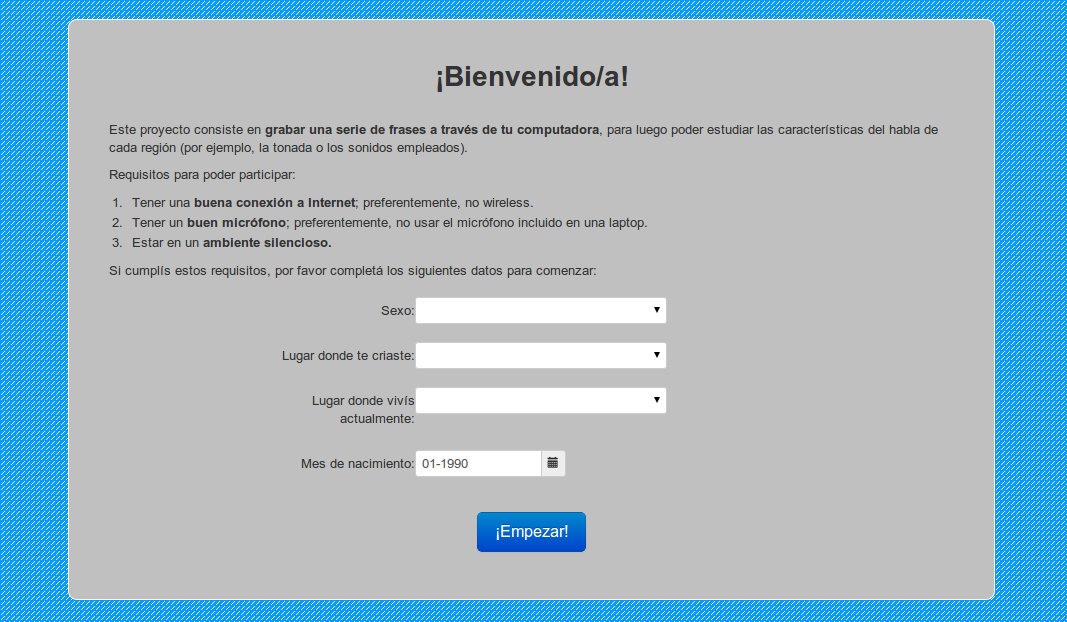
\includegraphics[width=0.8\textwidth]{pag-inicio2} }
    \caption{Encuesta inicial del sistema}
    \label{figEncuesta}
\end{figure}

\begin{figure}[h!]
    \centerline{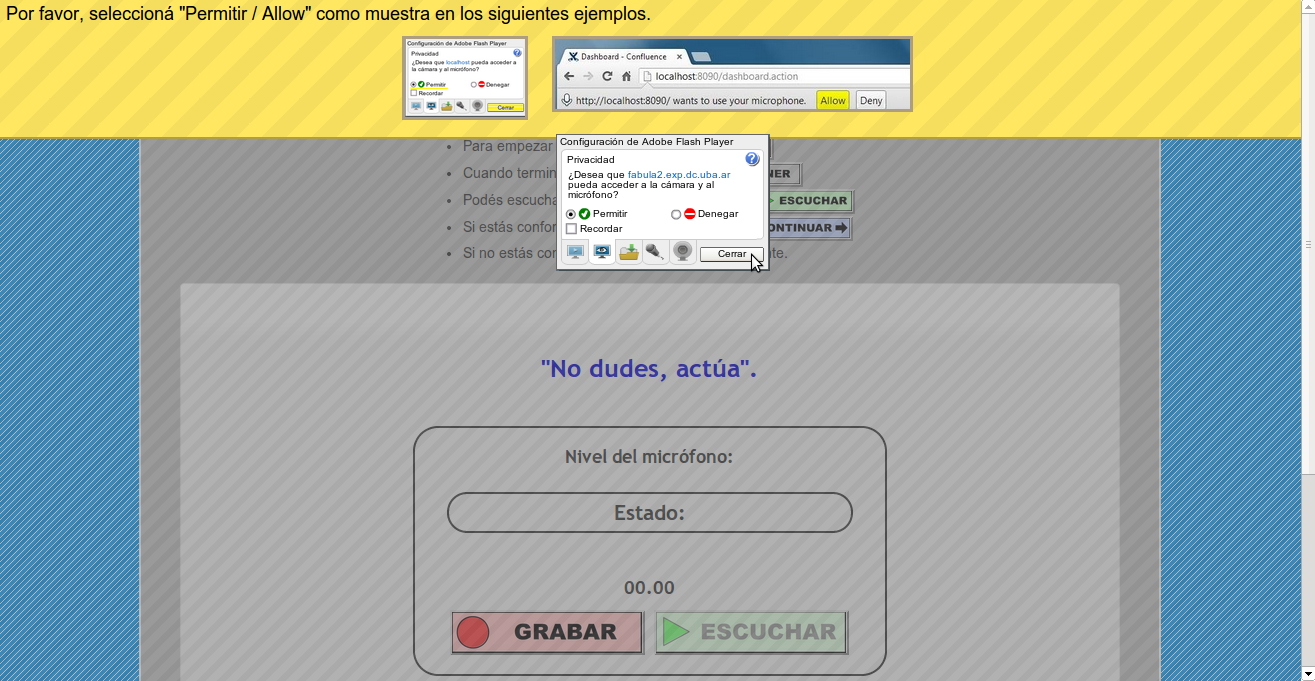
\includegraphics[width=0.8\textwidth]{pag-allow1} }
    \caption{Se debe permitir micrófono para comenzar el experimento}
    \label{allowmic}
\end{figure}

\begin{figure}[h!]
    \centerline{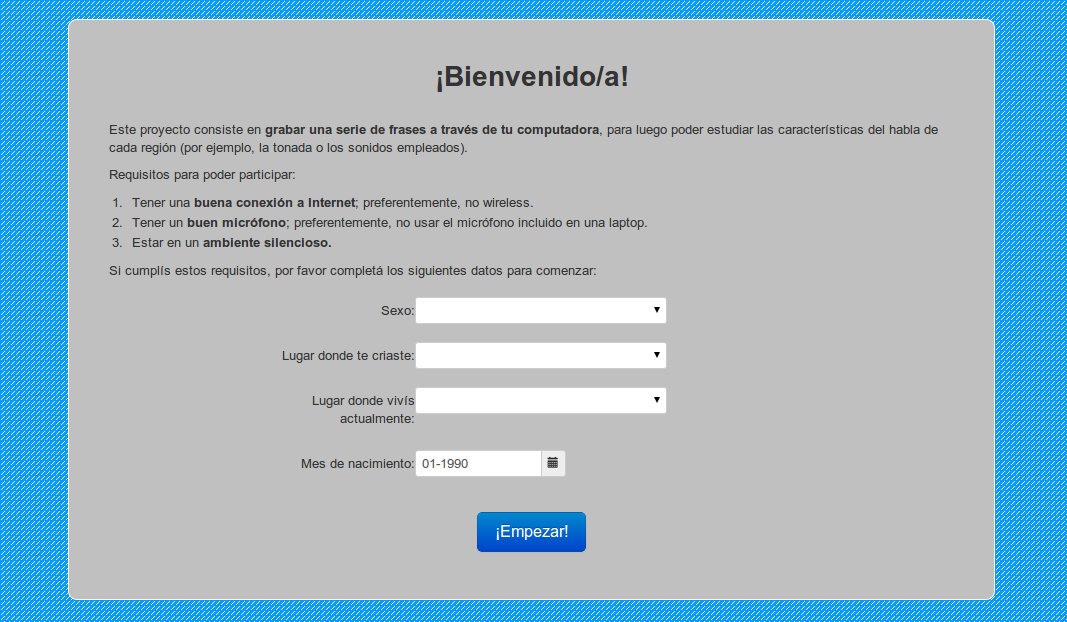
\includegraphics[width=0.8\textwidth]{pag-inicio2} }
    \caption{Inicio del experimento}
    \label{inicio}
\end{figure}

\begin{figure}[h!]
    \centerline{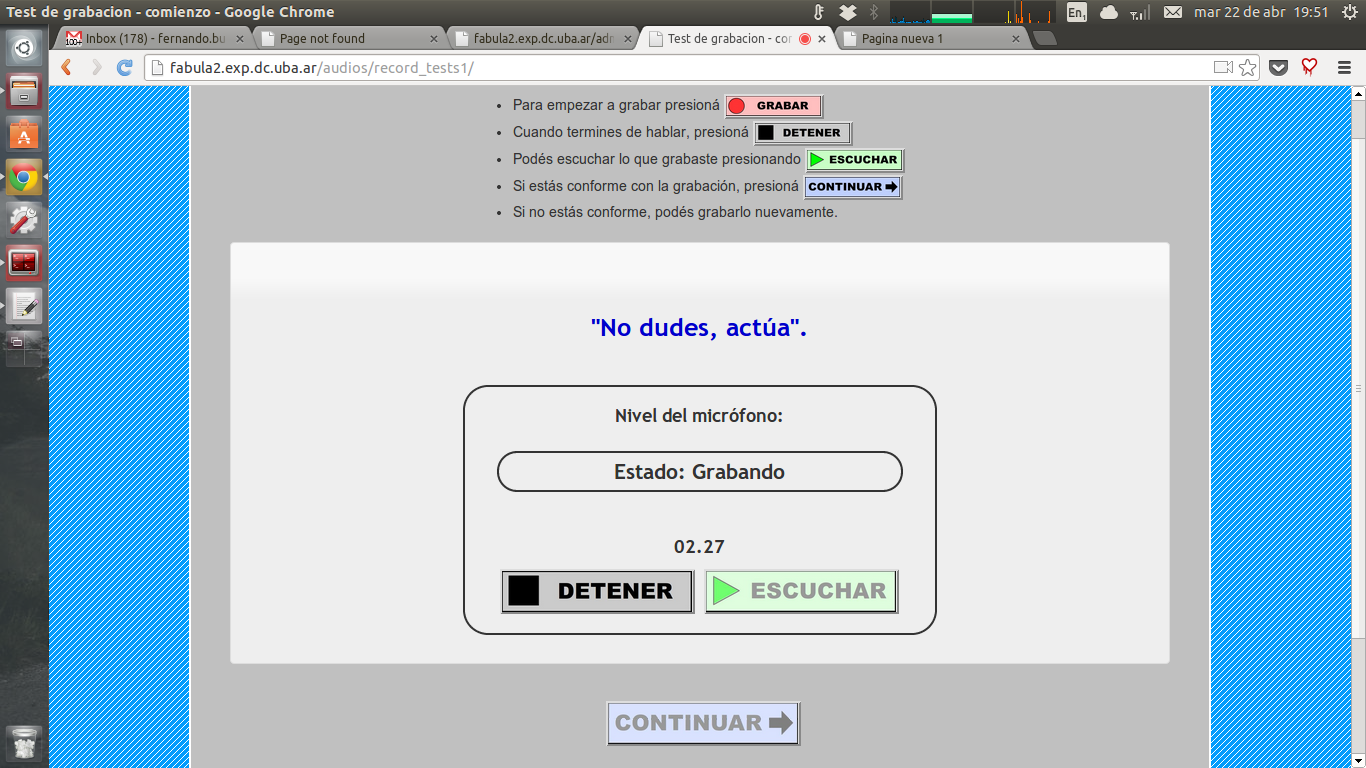
\includegraphics[width=0.8\textwidth]{pag-grabar1} }
    \caption{Grabando una frase}
    \label{grabando}
\end{figure}

\begin{figure}[h!]
    \centerline{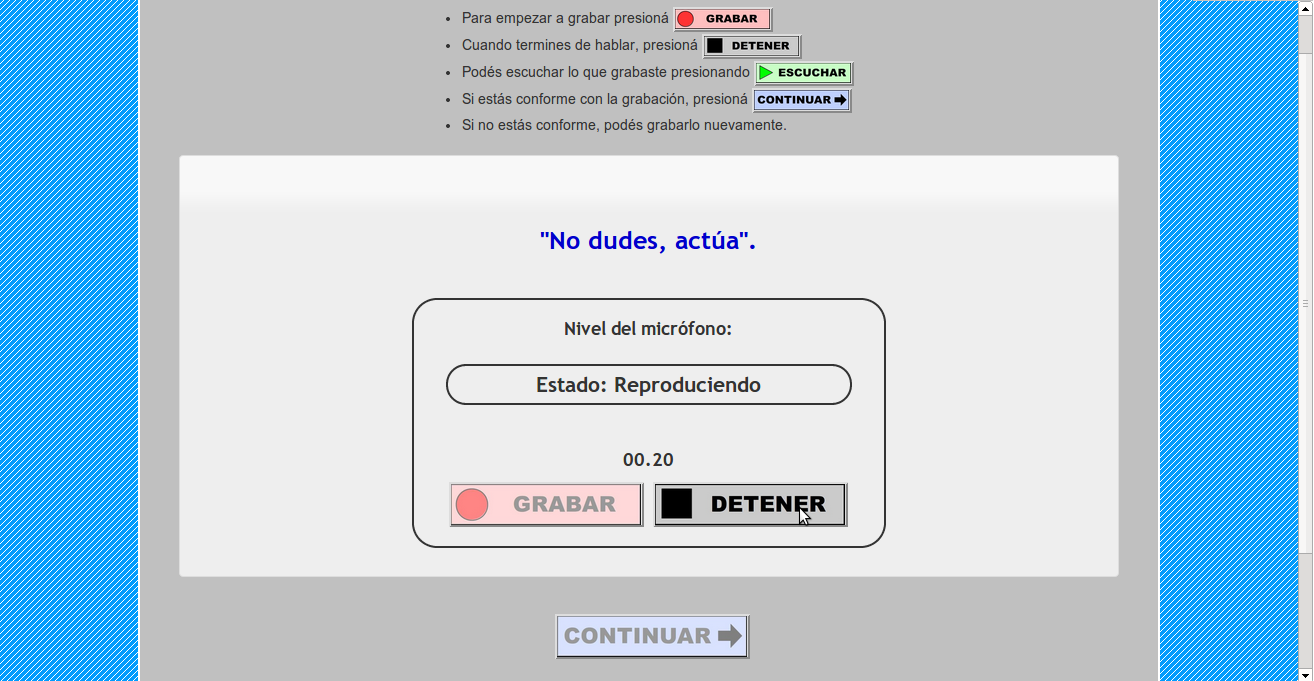
\includegraphics[width=0.8\textwidth]{pag-play1} }
    \caption{Reproduciendo la frase anteriormente grabada}
    \label{reproduciendo}
\end{figure}

En la pantalla de grabación el usuario debió confirmar tener acceso al micrófono que posee en su dispositivo como se puede apreciar en la Figura \ref{allowmic}. Una vez hecho esto, se le explicó las instrucciones como se ve en la Figura \ref{inicio} y luego puede empezar a grabar. 

Cada nuevo experimento utilizó una nueva traza del conjunto de trazas descriptas en la capitulo anterior. La interfaz que vio el usuario al grabar se puede ver en la Figura \ref{grabando}. Las grabaciones pueden ser escuchadas antes de ser confirmadas por el usuario. Lo importante es que la grabación se escuchen lo mejor posible. Para reproducir se aprieta en el botón \textit{Reproducir} como se ve en Figura \ref{reproduciendo}. 

Una vez que el hablante chequeó que su grabación se escucha bien, la confirma. Cada vez que se graba un audio, esta se guarda en un archivo wav en el servidor. El archivo que se genera tiene una frecuencia de muestreo de 22050 Hz, cada muestra se analiza con 16 bits y posee un solo canal. Con estas características pudimos obtener un audio de buena calidad para el experimento que realizamos.

Recordemos que los hablantes fueron grabando cada 5 frases. Una vez terminado estas 5 frases se le preguntó si quiere seguir grabando o terminar el experimento. De esta forma, aporta el tiempo que el hablante pudo disponer.

\section{Grabación a través del browser}

Los navegadores actuales no pueden soportar acceder al micrófono directamente. Durante la tesis se desarrolló HTML5 que podrá soportar acceder al micrófono y a recursos similares de forma más fácil. No se eligió basarse en este porque sólo algunos browsers lo soportaban. Al ser un estándar muy nuevo necesita que el usuario tenga instalada últimas versiones de software y utilizarlo hubiera excluido mucha gente. Teniendo en cuenta esto debimos utilizar una tecnología alternativa. 

Encontramos un proyecto llamado Web Accessible Multimodal Interfaces \footnote{Página web: https://code.google.com/p/wami/}. WAMI es una aplicación Flash que nos permite acceder al micrófono a través de JavaScript. El proyecto WAMI es muy utilizado en proyectos similares procesamiento de habla. Esta herramienta nos permite configurar dos urls importantes: una que se utilizará para enviar el audio grabado y otra para escucharlo.  

Cuando termina de grabar, se envía un mensaje POST al servidor a la url configurada. El servidor obtiene el paquete de información y lo guarda como archivo wav. Cuando se quiere reproducir algún audio se envía un mensaje GET a la otra url. El servidor lo responde con el audio requerido y se reproduce en el navegador. También con WAMI se puede configurar la calidad del audio grabado y analizar el nivel del volumen que posee. 

\subsection{Requerimientos}

Los requerimientos para participar del experimento fueron básicos: micrófono y conexión a internet. Tuvimos problemas sobre el browser que se utilizaba: WAMI necesita Flash versión 11.04 que no se encuentra en los repositorios tradicionales de Ubuntu. De esta manera, los navegadores que utilicen Flash instalado por el sistema operativo Ubuntu no podrán correr. Otros sistemas operativos como Windows o MacOs no tienen problemas en la versión de Flash instalada. De todas formas el navegador Chrome posee preinstalado la última versión de Flash, quiere decir que este navegador puede correr perfectamente la aplicación sin importar el sistema operativo que se utilice.

\section{Varias grabaciones por frase}

Siguiendo con la idea de tener la mejor grabación de cada hablante, le dimos la opción a cada hablante que después de grabar un audio de una frase puedan escucharse como quedó. Esto requiere un ida y vuelta de paquetes entre el cliente (navegador) y el servidor. 

Como dijimos anteriormente, al grabar el cliente manda un mensaje al servidor con el audio de la grabación en crudo. Las frases son de corta longitud entonces no es necesario preocuparse por la longitud del paquete. Cuando el cliente quiere escucharlo envía un mensaje pidiendo ese mismo audio anteriormente grabado. El servidor envía el audio y es reproducido en el cliente. Esta ida y vuelta de la grabación podría ser optimizada para que la grabación pueda ser escuchada sin tener interacción con el servidor. En nuestro experimento, no tuvimos problemas graves en lo que respecta a latencias pero si es un punto débil del sistema que hay que tener en cuenta.

Puede resultar interesante analizar los anteriores audios grabados y porque el hablante se queda con el último. Esta idea también puede motivar a algún trabajo futuro. Este es otro motivo porque lo realizamos.

\section{Sistema de administración}

Además de la interfaz pública para grabar audios, implementamos un sistema privado para administrar las grabaciones. Este nos permite ver las grabaciones que fueron grabadas, la cantidad de grabaciones por cada frase que tenemos recolectada, la cantidad de trazas que todavía no se utilizaron, entre otras cosas. También vamos a poder escuchar y marcar las grabaciones para utilizarlas como primer filtro de las grabaciones. Explicaremos esto en mas detalle a continuación.

\subsection{Etiquetando audios}

Cuando varias personas terminan el experimento, los administradores pueden acceder a una página donde se puede escuchar cada audio que se va grabando. Los administradores escucharon los audios y según su calidad los etiquetaron con alguna de las etiquetas definidas. Las etiquetadas utilizadas esta vez son: `Conservar’,  `Sonido saturado’, `Mucho ruido de fondo’, `Problemas en el habla’. Esto se puede ver en Figura \ref{cat}.

\begin{figure}[h!]
    \centerline{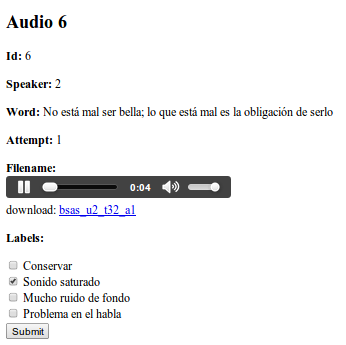
\includegraphics[width=0.5\textwidth]{categorizando_audios} }
    \caption{Categorizando audios}
    \label{cat}
\end{figure}

Para acceder a los audios que fueron etiquetados de una determinada manera, el sistema tiene distintas urls que nos permitieron bajar todos esos audios en un archivo de tipo tar. Entonces si quisiéramos bajarnos todos los audios etiquetados con la categoria `Conservar’ podemos acceder a una url y bajarnos sin necesidad de entrar al servidor. Se necesita ser usuario del sistema para poder acceder aquí.

\section{Backups automáticos}

El sistema posee backups que se generan a la noche automáticamente. Los backups consisten en un volcado de información de toda la base de datos y en la sincronización de los audios con una carpeta externa de backup. De esta forma, se guardan todos los datos cada día, y quedan a salvo.

\section{Análisis del volumen}

Un objetivo primordial de este experimento es evitar grabaciones saturadas. Para ello se nos ocurrió medir el volumen de la grabación cuando sucede la misma. El resultado es una serie de valores entre 0 a 100. Sobre estos valores vamos a calcular el máximo y el mínimo. Si el primero es mayor a un cierto umbral (o sea mayor a 80 por ejemplo) quiere decir que en la grabación se saturó en algún momento. Si el mínimo es mayor a un cierto umbral (o sea menor a 20 por ejemplo) quiere decir que hay mucho sonido ambiente. En cualquiera de los dos casos podemos pedirle al usuario que grabe de vuelta el experimento. De esta forma podemos filtar audios que no nos servirán para reconocer el acento.

Si bien esta característica fue programada, no fue utilizada en la recolección de datos. El motivo fue que queríamos chequear cuan bien funcionaba la herramienta sin filtros y con completa participación de los usuarios. Otro motivo fue la paciencia de los hablantes. Puede suceder que al tratar de grabar no logre un ambiente beneficioso para grabar. Esto quiere decir que aunque quiera grabar el filtro rechace todos sus audios. También notamos que había grabaciones que dieron mal el filtrado del volumen pero la grabación era buena. Esto no lo queremos como primer experimento del framework. Por eso elegimos aceptar todos sus audios.

A continuación veremos como utilizamos esta información recolectada para el objetivo del experimento.